\documentclass{fitj}
\usepackage[dvipdfmx]{graphicx}
\usepackage{amsmath}
\usepackage{txfonts}
\usepackage{pifont}
\usepackage{url}
\usepackage{multirow}
\usepackage{hhline}
\usepackage[dvipdfmx,hidelinks]{hyperref}
% \def\labelenumi{(\theenumi)}

\setlength{\textfloatsep}{6pt plus 1pt minus 2pt}
\setlength{\floatsep}{6pt plus 1pt minus 2pt}
\setlength{\intextsep}{6pt plus 1pt minus 2pt}

\bibliographystyle{junsrt}

% 和文タイトル-----------------------------------------------------------------
\jtitle{協調認識のための交通流予測に基づく\\帯域適応型V2Xハイブリッド経路制御方式の検討}
%---------------------------------------------------------------------------

% 英文タイトル-----------------------------------------------------------------
\etitle{Bandwidth-Adaptive V2X Hybrid Routing Control\\Based on Traffic Flow Prediction for Cooperative Perception}
%---------------------------------------------------------------------------

% 著者数：著者の数だけ c を書く---------------------------------------------------
\authors{cccc}
%---------------------------------------------------------------------------

% 和文著者名：著者名間に & を書く------------------------------------------------
\jauthors{古米 遼成\dag & 末澤 智崇\ddag & Onur Alparslan\S & 佐藤 健哉\ddag\S}
%---------------------------------------------------------------------------

% 欧文著者名：著者名間に & を書く------------------------------------------------
\eauthors{Ryosei Furumai & Satoshi Suezawa & Onur Alparslan & Kenya Sato}

%\pagestyle{plain}
%\setcounter{page}{7}

\begin{document}

\maketitle

% 所属
\footnotetext{{\dag} 同志社大学 理工学部 情報システムデザイン学科　Faculty of Science and Engineering, Doshisha University}
\footnotetext{{\ddag} 同志社大学大学院 理工学研究科 情報工学専攻　Information and Computer Science, Graduate School of Science and Engineering, Doshisha University}
\footnotetext{{\S} 同志社大学モビリティ研究センター　Mobility Research Center, Doshisha University}

%---------------------------------------------------------------------

%---------------------------------------------------------------------

\section{はじめに}
自動運転車両の安全性向上において，車載センサで得た周辺物標情報をCollective Perception Message（CPM）として共有する協調認識サービスが注目されている．また，路側機（Road Side Unit: RSU）が下流の交通状況や危険情報を上流車両へ事前通知する安全走行支援システムが検討されており\cite{soumu2025}，車車間通信（Vehicle-to-Vehicle: V2V）およびセルラ網の活用が求められている． 

しかし，車両密集環境においては，膨大なCPMの送信により無線チャネルが逼迫し，パケット衝突や遅延に伴う協調認識性能の低下を招く．従来のチャネル混雑度（Channel Busy Ratio: CBR）に基づく反応型混雑制御では，現在観測されたCBRに応じて送信制御を行うため\cite{etsidcc}，車両群の流入に伴って高負荷となる区間が時間的に変化する環境では対応が遅れ，突発的な通信品質の劣化を招く恐れがある．

そこで本稿では，車両密集環境における突発的な通信品質劣化を抑制し，協調認識率を維持・向上することを目的とし，上流交通流情報に基づくCBR予測方式，および物標重要度に基づく帯域適応型ハイブリッド経路制御方式を提案する．

\section{関連研究}
山崎らは，歩行者情報が冗長性緩和ルール（Redundancy Mitigation Rules: RMR）により削除されると歩行者認識率が低下する点に着目し，歩行者情報を優先的にCPMへ含めるRMRを提案した\cite{yamasaki2023}．この方式は歩行者認識率を維持しつつV2V負荷を低減できる一方，下流混雑の先読みや別経路による補完は対象外であり，突発的な通信品質劣化が発生する可能性がある．

\section{提案方式}

\subsection{概要}
本方式では，物標重要度を距離，接近速度および衝突余裕時間（Time To Collision: TTC）に基づいて定義する．図\ref{fig:proposal_overview}に示すように，RSU間で共有した上流交通流情報から予測CBRを算出し，車両は予測CBRと物標重要度に基づいてV2V経路と，MEC（Multi-access Edge Computing）を介したV2N2V経路を選択する．

  \begin{figure}[t]
    \centering
    
\includegraphics[width=\linewidth]{概要図.png}
    \caption{$\hat{C}_{n}$ が制御閾値以下の場合の提案方式}
    \label{fig:proposal_overview}
  \end{figure}

\subsection{RSU間連携による下流混雑の先読み方式}
本方式では，上流RSUで観測された車両群の位置，速度，CPM送信量をRSU間で共有し，車両群が下流区間へ流入した際のCBRを予測する．

各RSUは周辺車両の位置，速度，CPM送信量および実測CBRを観測する．下流RSUは，上流RSUから共有された交通流情報を用い，予測時間窓内に自区間へ流入する車両数を算出する．区間$n$における予測CBR $\hat{C}_{n}$ を次式で定義する．
\begin{equation}
{\small
\hat{C}_{n} = \min \left( 1, \max(C^{\mathrm{m}}_{n},C^{0}_{n}) + \max(0,C^{\mathrm{f}}_{n}-C^{0}_{n}) \right)
}
\end{equation}
\begin{equation}
 C^{\mathrm{f}}_{n} = \frac{N^{\mathrm{f}}_{n}\lambda \bar{S}}{R}
\end{equation}
ここで，$C^{\mathrm{m}}_{n}$は通常のCPMに加え，各車両が発生させる背景トラフィックも含め実測したCBR，$C^{0}_{n}$は現在の車両数から算出したCBR，$C^{\mathrm{f}}_{n}$は予測流入車両数$N^{\mathrm{f}}_{n}$が発生させるCBRであり，$\lambda$はCPM送信頻度，$\bar{S}$は平均CPMサイズ，$R$はチャネル伝送速度である．式(1)では実測値と算出値の大きい方を基準とし，将来流入で増加する負荷分のみを加えることで，負荷の過小評価を避ける．

\subsection{物標重要度に基づく帯域適応型経路制御方式}
車両は通知された予測CBRと，自車センサが捉えた各物標の重要度に基づいて通信経路を動的に決定する．近距離，または短時間で接近する事故リスクの高い物標を「高重要度」と判定する．混雑環境下における高重要度情報の未達は安全性低下に直結する可能性があるため，V2VとV2N2Vの双方の通信経路を用いて二重送信を行い，到達信頼性を向上させる．

一方，それ以外の低重要度情報は，予測CBR $\hat{C}_{n}$ に応じた確率でV2N2V経路にも転送し，V2V単独では認識困難な物標情報の到達性を補完する．低重要度情報をV2N2V経路にも転送する確率 $p_{\mathrm{L}}$ を次式で定義する．
\begin{equation}
{\small
p_{\mathrm{L}} =
\begin{cases}
p_{\mathrm{L,max}}, & \hat{C}_{n} \le C_{\mathrm{switch}}, \\[2pt]
p_{\mathrm{L,max}}\dfrac{C_{\max}-\hat{C}_{n}}{C_{\max}-C_{\mathrm{switch}}}, & C_{\mathrm{switch}}<\hat{C}_{n}<C_{\max}, \\[2pt]
0, & \hat{C}_{n} \ge C_{\max}.
\end{cases}}
\end{equation}
ここで，$p_{\mathrm{L,max}}$は低重要度情報のV2N2V転送確率の上限値である．予測CBRが高い場合には，高重要度情報を優先するため，低重要度情報の転送確率を低下させる．

\section{評価}

\subsection{評価環境}
Van3Twinを用い，ns-3およびSUMOを統合した3\,kmの双方向6車線高速道路シナリオを構築した．予測時間窓は，RSU間隔約500\,mを平均速度約25\,m/sで走行する時間相当の20\,sとした．主な評価条件を表\ref{tab:condition}に示す．

\begin{table}[t]
\centering
\caption{主な評価条件}
\label{tab:condition}
\small
\begin{tabular}{cc}
\hline
項目 & 設定値 \\ \hline \hline
シミュレーション時間 & 120\,s \\
総車両数 / 通信車両数 & 250 / 100 \\
RSU数 & 6 \\
V2V通信方式 & NR-V2X sidelink \\
センサ範囲 / 評価範囲 & 100 / 200\,m \\
交通流予測時間窓 & 20\,s \\
I2V通知範囲 & 300\,m \\
高 / 低重要度情報の有効時間 & 0.2 / 0.5\,s \\
高重要度判定距離 / 速度 / TTC & 50\,m / 3\,m/s / 5\,s \\
制御閾値 $C_{\mathrm{switch}}$ / $C_{\max}$ & 0.6 / 0.8 \\
転送確率上限 $p_{\mathrm{L,max}}$ & 0.5 \\
MEC遅延中央値 / p99 / PDR & 49 / 84\,ms / 0.97 \\ \hline
\end{tabular}
\end{table}

評価指標には，評価範囲内の物標を有効時間内に認識できた割合である周辺物標認識率（ORR），重要度別ORR，平均CBR，および送信データ量を採用した．比較方式として無制御，現在CBRに基づく冗長情報削減（反応型RMR），予測CBRに基づく冗長情報削減（予測RMR），低重要度情報の二重送信を行わず高重要度情報のみを二重送信する方式，提案方式（適応型V2N2V）の5方式を評価した．

\subsection{評価結果および考察}
120秒間のシミュレーションにおける各方式の比較結果を図\ref{fig:result_graph}に示す．

\begin{figure}[t]
\centering

\includegraphics[width=\columnwidth]{result_graph.pdf}
\caption{各方式における周辺物標認識率（ORR）と平均CBR（百分率表示）の比較結果}
\label{fig:result_graph}
\end{figure}

\begin{figure}[t]
\centering
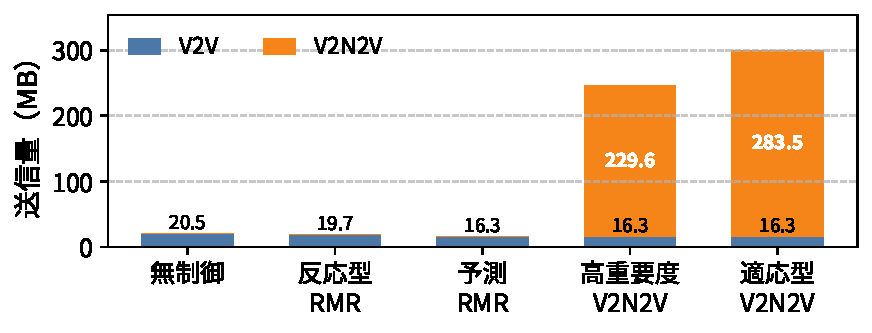
\includegraphics[width=\columnwidth]{transmission_volume_graph.pdf}
\caption{各方式におけるV2VおよびV2N2V送信量の比較結果}
\label{fig:transmission_volume}
\end{figure}

評価結果では，適応型V2N2Vは高重要度ORRを99.68\%で維持しつつ，低重要度ORRを無制御の38.74\%から87.47\%へ向上し，全体ORRを91.59\%へ引き上げた．これは，高重要度情報の二重送信に加え，予測CBRを低重要度情報のV2N2V転送確率制御に用いることで，将来のV2V混雑を考慮しつつ未受信物標を補完できたためである．

反応型RMRおよび予測RMRは，無制御と同程度の全体ORRを維持したまま平均CBRを低減した．これは，認識率への寄与が小さい冗長な物標情報を削減し，CPMサイズおよびV2V送信量を抑制したためである．また，図\ref{fig:transmission_volume}に示すように，両RMRはORRの差が小さい一方でV2V送信量を削減しており，RMRの主目的はORRを維持したV2V負荷の抑制にある．

ただし，本評価ではMEC経路の遅延およびPDRを表\ref{tab:condition}の固定条件として与えており，V2N2V送信量増加に伴うセルラ網側の輻輳は考慮していない．また，本評価環境では予測CBRに基づくRMR単独では反応型RMRとの差は限定的であったが，予測CBRをV2N2V転送確率制御に用いることで，将来のV2V混雑を考慮した補完送信が可能となった．CBRが急変する環境での評価は今後の課題である．

\section{まとめ}
本研究では，車両密集環境における突発的な通信品質劣化の課題に対し，予測CBRと物標重要度に基づいてV2V/V2N2V経路を動的に選択する方式を提案した．評価の結果，予測CBRに基づく経路制御によりV2Vのチャネル負荷を抑制しつつ，V2N2V経路により全体ORRを向上できることを示した．

%---------------------------------------------------------------------

%---------------------------------------------------------------------

\section*{謝辞}
本研究の一部はJSPS科研費JP24H00698の助成を受けたものである．

%----------------------------------------------------------------------

%----------------------------------------------------------------------
{\footnotesize 
\begin{thebibliography}{99}
  \bibitem{soumu2025} 
  総務省, “自動運転に係る情報通信インフラの取組について”, 第3回自動運転インフラ検討会資料 (2025).

  \bibitem{etsidcc} 
  ETSI, “Intelligent Transport Systems (ITS); Decentralized Congestion Control Mechanisms”, ETSI TS 102 687, Vol.1, No.2 (2011).

  \bibitem{yamasaki2023} 
  山崎 慎也, “車両の走行環境を考慮した協調認識メッセージにおける冗長性緩和手法”, 同志社大学修士論文 (2023).
\end{thebibliography}
}
\end{document}
%---------------------------------------------------------------------
